\section{Aufbau}
\label{sec:aufbau}
\subsection{Gerätedaten}
Für alle Messungen wurde Gerät 2 verwendet mit folgenden Spezifikationen:\\
$L= (10,11\pm 0.03)\;\symup{mH}$, $C=(2,098 \pm 0.006)\;\symup{nF}$,
$R_1 =(48,1 \pm 0,1)\; \symup{\Omega}$, $R_2=(509,5 \pm 0,5)\;\symup{\Omega}$

\subsection{Messapparatur zur Bestimmung des Dämpfungswiderstandes}
\label{ssec:a12}
Die ersten beiden Messreihen zur Bestimmung des Dämpfungswiderstandes
werden mit einer Schaltung, wie in Abbildung \ref{fig:5a}, verwirklicht.
Der Aufbau unterscheidet sich für die Messreihen nur dahingehend, dass
für die Bestimmung des Dämpfungswiderstandes für den aperiodischen Grenzfall
der Widerstand R durch einen regelbaren Wiederstand ausgetauscht wird.
\begin{figure}
  \centering
  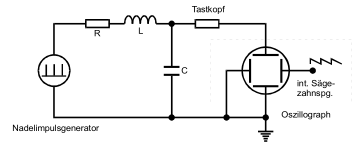
\includegraphics[height= 4cm]{./logos/Amplitude_Schaltung.PNG}
  \caption{Zur Erfassung der Schwingung des angeregten RCL-Kreises verwendete
  Schaltung mit $R = R_1$ aus Quelle \cite{sample}}
  \label{fig:5a}
\end{figure}
\FloatBarrier
\subsection{Messapparatur zur Bestimmung der Frequenzabhängigkeit...}
\subsubsection{...der Kondensatorspannung}
Zur Messung der Frequenzabhängigkeit der am Kondensator auftretenden Spannung
stellt man den Impulsgenerator aus Abb.\ref{fig:5a} so um, dass er eine
Sinusspannung generiert. Desweiteren wird $R=R_2$ gewählt.
\subsubsection{...der Phase zwischen Erreger-und Kondensatorspannung}
\label{sssec:a4}
Wieder gilt $R=R_2$. Die Messapparatur für diesen Teil des Versuches
unterscheidet sich von der aus Teil \label{sec:a12} nur dahingehend, dass
die Sinusspannung des Generators auf den Zweitkanal des Oszillographs gelegt
wird.
\subsubsection{...des Scheinwiederstandes}
Ist gleich der aus Teil \ref{sssec:a4}.
